\documentclass[a4paper,12pt]{article}
\usepackage[T1,T2A]{fontenc}
\usepackage[utf8]{inputenc}
\usepackage[english,ukrainian]{babel}


\usepackage{ upgreek }
\usepackage{amsmath}

\usepackage{graphicx}
\graphicspath{{./pictures/}}


\usepackage[unicode=true,colorlinks=true,urlcolor=blue,citecolor=green,linkcolor=blue]{hyperref}
\usepackage[ukrainian,nameinlink]{cleveref}
\usepackage{geometry} % Меняем поля страницы
\geometry{left=2cm}% левое поле
\geometry{right=1.5cm}% правое поле
\geometry{top=1cm}% верхнее поле
\geometry{bottom=2cm}% нижнее поле



\begin{document}
	
	\begin{titlepage}
		\vspace*{6cm}
		\begin{center}
			
			\large
			\textbf{Звіт}\\
			\textbf{до лабораторної роботи №3:}\\
			\textbf{<<Чисельне моделювання в’язкої ньютонівської нестислої рідини.>>}
			
		\end{center}
		
		\vspace{8cm}
		\begin{flushright}
			студента 1-го курсу магістратури\\
			факультету комп'ютерних наук та кібернетики\\
			Кравця Олексія
		\end{flushright}
		
	\end{titlepage}

\newpage
\tableofcontents
\newpage
\section{Постановка задачі}

Для моделювання будемо використовувати лінеаризовану систему рівнянь Нав'є-Стокса.

\begin{equation} \label{eq1.1}
	\frac{\partial u}{\partial t} = - \frac{1}{\rho} \frac{\partial p}{\partial x} + \nu \left( \frac{\partial^2 u}{\partial x^2} + \frac{\partial^2 u}{\partial y^2} \right)
\end{equation}

\begin{equation} \label{eq1.2}
\frac{\partial v}{\partial t} = - \frac{1}{\rho} \frac{\partial p}{\partial y} + \nu \left( \frac{\partial^2 v}{\partial x^2} + \frac{\partial^2 v}{\partial y^2} \right)
\end{equation}

\begin{equation} \label{eq1.3}
	\frac{\partial u}{\partial x}+ \frac{\partial v}{\partial y} = 0, \quad (x,y) \in \Omega = \{ 0\le x \le a, 0 \le y \le d \}, \; t > 0
\end{equation}

Де $u(x,y,t)$ -- складова швидкості по осі $x$, $v(x,y,t)$ -- складова швидкості по осі $y$, $p(x,y,t)$ -- тиск. $\rho$ -- густина, $\nu$ -- кінематичний коефіцієнт в'язкості.

Маємо наступні початкові умови:

\begin{equation} \label{eq1.4}
	u|_{t =0} = u^0(x,y); \quad v|_{t = 0} =v^0(x,y); \quad p|_{t=0} =p^0(x,y)
\end{equation}
та граничні умови (першого роду):
\begin{equation}\label{eq1.5}
	\begin{aligned}
		&u|_{x = 0} = u^0 (y,t); \quad v|_{x=0} = v^0(y,t); \quad p|_{x = 0} = p^0(y,t);\\
		&u|_{x = a} = u^a(y,t); \quad v|_{x=a} = v^a(y,t); \quad p|_{x = a} = p^a(y,t);\\
		&u|_{y = 0} = u^0 (x,t); \quad v|_{y=0} = v^0(x,t); \quad p|_{y = 0} = p^0(x,t);\\
		&u|_{y = d} = u^d (x,t); \quad v|_{y=d} = v^d(x,t); \quad p|_{y = d} = p^d(x,t);
	\end{aligned}
\end{equation}
Також дано точний розв'язок:

\begin{equation} \label{eq1.6}
	\begin{aligned}
		&u(x,y,t) = - e^{-t} e^{\frac{2y}{d}} \sin \left( \frac{2x}{d} \right)\\
		&v(x,y,t) = e^{-t} e^{\frac{2y}{d}} \cos \left( \frac{2x}{d} \right) \\
		&p(x,y,t) = \frac{d}{2} \rho e^{-t} e^{\frac{2y}{d}} \cos \left( \frac{2x}{d} \right)
	\end{aligned}
\end{equation}
Саме з формул (\ref{eq1.6}) обраховуються формули (\ref{eq1.4}), (\ref{eq1.5}).

Необхідно побудувати динаміку зміни векторного поля швидкостей, а також динаміку зміни тиску. Порівняти обчислений розв'язок з точним.

\section{Опис чисельного методу}
Позначимо $\tau$ -- часовий крок, $h_x$ -- крок по осі $x$, $h_y$ -- крок по осі $y$.

Якщо (\ref{eq1.1}) продиференціювати по $x$, а (\ref{eq1.2}) -- по $y$, і скласти отримані рівняння, х врахуванням (\ref{eq1.3}), отримаємо рівняння Пуасона для тиску

\begin{equation} \label{eq2.1}
	\frac{\partial^2 p}{\partial x^2} + \frac{\partial^2 p}{\partial y^2} = - \frac{\partial D}{\partial t} + \frac{1}{Re} \left( \frac{\partial^2 D}{\partial x^2} + \frac{\partial^2 D}{\partial y^2} \right), \quad \text{де} \; D = \frac{\partial u}{\partial x} + \frac{\partial v}{\partial y}
\end{equation}
Рівняння (\ref{eq2.1}) можна апроксимувати на п'яти-точковому шаблоні.
\begin{equation} \label{eq2.2}
	\Delta_h p^{n+1}_{i,j} = S^{n}_{i,j}
\end{equation}
де
\begin{equation} \label{eq2.3}
	S_{i,j}^{n} = \frac{D_{i,j}^n}{\tau} + \frac{1}{Re} \Delta_h D_{i,j}^n
\end{equation}
Тут
\begin{equation} \label{eq2.4}
	\begin{aligned}
	&D_{i,j}^n = L_1 u_{i,j}^n + L_2 v_{i,j}^n \\
	&L_1 u_{i,j}^n = \frac{u_{i+1,j}^n - u_{i-1,j}^n}{2h_x}\\
	&L_2 v_{i,j}^n = \frac{v_{i,j+1}^n - v_{i,j-1}^n}{2h_y}\\
	&\Delta_h p^n_{i,j} =\frac{p^{n}_{i+1,j} - 2 p^{n}_{i,j} + p^{n}_{i-1,j}}{h_x^2} + \frac{p^{n}_{i,j+1} - 2 p^{n}_{i,j} + p^{n}_{i,j-1}}{h^2_y}
	\end{aligned}
\end{equation}

Зауважимо, що у своїх розрахунках я змінив формулу (\ref{eq2.3}) та знехтував доданком з числом Рейнольдса.
\begin{equation} \label{eq2.5}
	S_{i,j}^{n} = \frac{D_{i,j}^n}{\tau}
\end{equation}

\subsection{Двокроковий симетризований алгоритм}

Для оновлення $u_{i,j}$, $v_{i,j}$ будемо використовувати двокроковий симетризований алгоритм. 

Давайте розглянемо точки $u^n_i,j$, для яких виконується $i+j+n \; \vdots\; 2$. Будемо оновлювати їх за явною різницевою схемою:

\begin{equation} \label{eq2.6}
	\frac{u^{n+1}_{i,j} - u^{n}_{i,j}}{\tau} = - \frac{1}{\rho} \frac{p^{n+1}_{i,j} - p^{n+1}_{i-1,j}}{2h_x}+ \nu \left( \frac{u^{n}_{i+1,j} - 2u^{n}_{i,j} + u^{n}_{i-1,j}}{h_x^2}  + \frac{u^{n}_{i,j+1} -2 u^{n}_{i,j} + u^{n}_{i,j-1}}{h_y^2}\right)
\end{equation}
Тепер розглянемо точки, що залишилися, тобто точки $u_{i,j}^n$ для яких $i+j+n$ не ділиться на $2$. Будемо оновлювати їх за неявною різницевою схемою:
\begin{equation} \label{eq2.7}
	\frac{u^{n+1}_{i,j} - u^{n}_{i,j}}{\tau} = - \frac{1}{\rho} \frac{p^{n+1}_{i,j} - p^{n+1}_{i-1,j}}{2h_x}+ \nu \left( \frac{u^{n+1}_{i+1,j} - 2u^{n+1}_{i,j} + u^{n+1}_{i-1,j}}{h_x^2}  + \frac{u^{n+1}_{i,j+1} -2 u^{n+1}_{i,j} + u^{n+1}_{i,j-1}}{h_y^2}\right)	
\end{equation}

Завдяки (\ref{eq2.6}) можемо явно розв'язати (\ref{eq2.7})
\begin{equation}	\label{eq2.8}
	u^{n+1}_{i,j} = u^{n}_{i,j} - \frac{\tau}{\rho} \frac{p^{n+1}_{i,j} - p^{n+1}_{i-1,j}}{2h_x} + \frac{\tau \nu \left(  \frac{u^{n+1}_{i+1,j}+u^{n+1}_{i-1,j}}{h_x^2} + \frac{u^{n+1}_{i+1,j}+u^{n+1}_{i-1,j}}{h_y^2}\right)}{1 + 2 \tau \nu \left( \frac{1}{h_x^2} + \frac{1}{h_y^2} \right)}
\end{equation}

Аналогічно можна знайти $v_{i,j}^{n+1}$.

\subsection{Алгоритм}

Чисельний метод знаходження $u,v,p$:

\begin{itemize}
	\item Знаходимо тиск $p^{n+1}$ з рівняння (\ref{eq2.2}) ітераційним методом верхньої релаксації \cite[стор.182-183]{Rouch}:
	\begin{equation}\label{eq2.9}
		p^{r+1}_{i,j} = p^{r}_{i,j} + \frac{w}{2(1+\beta^2)} \left[ p^{r}_{i+1,j} + p^{r+1}_{i-1,j} + \beta^2 p^{r}_{i,j+1} + \beta^2 p^{r+1}_{i,j-1} - h_x^2 S_{i,j} - 2(1+ \beta^2) p^{r}_{i,j}\right]
	\end{equation}
	де $\beta = \frac{h_x}{h_y}$, $r = 1,2,\ldots$ -- номер ітерації. Часовий індекс $n$ опущений для спрощення запису. $w$ -- параметр релаксації $1 \le w \le 2$, його обраховуємо автоматично по формулам з \cite{Rouch}.
	\item Компоненти швидкості $u^{n+1}$, $v^{n+1}$ знаходимо, використовуючи двокроковий симетризований алгоритм. Формули (\ref{eq2.6} - \ref{eq2.8}).
\end{itemize}

\section{Результати}

Візьмемо такі параметри:
\[
	\begin{aligned}
		&a = 3.1; \quad d = 1; \\
		&h_x = 0.1; \quad h_y = 0.1;\\
		&t_0 =0; \quad \tau= 0.1;\\
		&\rho =1; \quad \nu = 1.		
	\end{aligned}
\]
Тоді після одного кроку роботи алгоритму та після $100$ кроків маємо такі результати (рис. \ref{ris:1})

\begin{figure}[h]
	\center 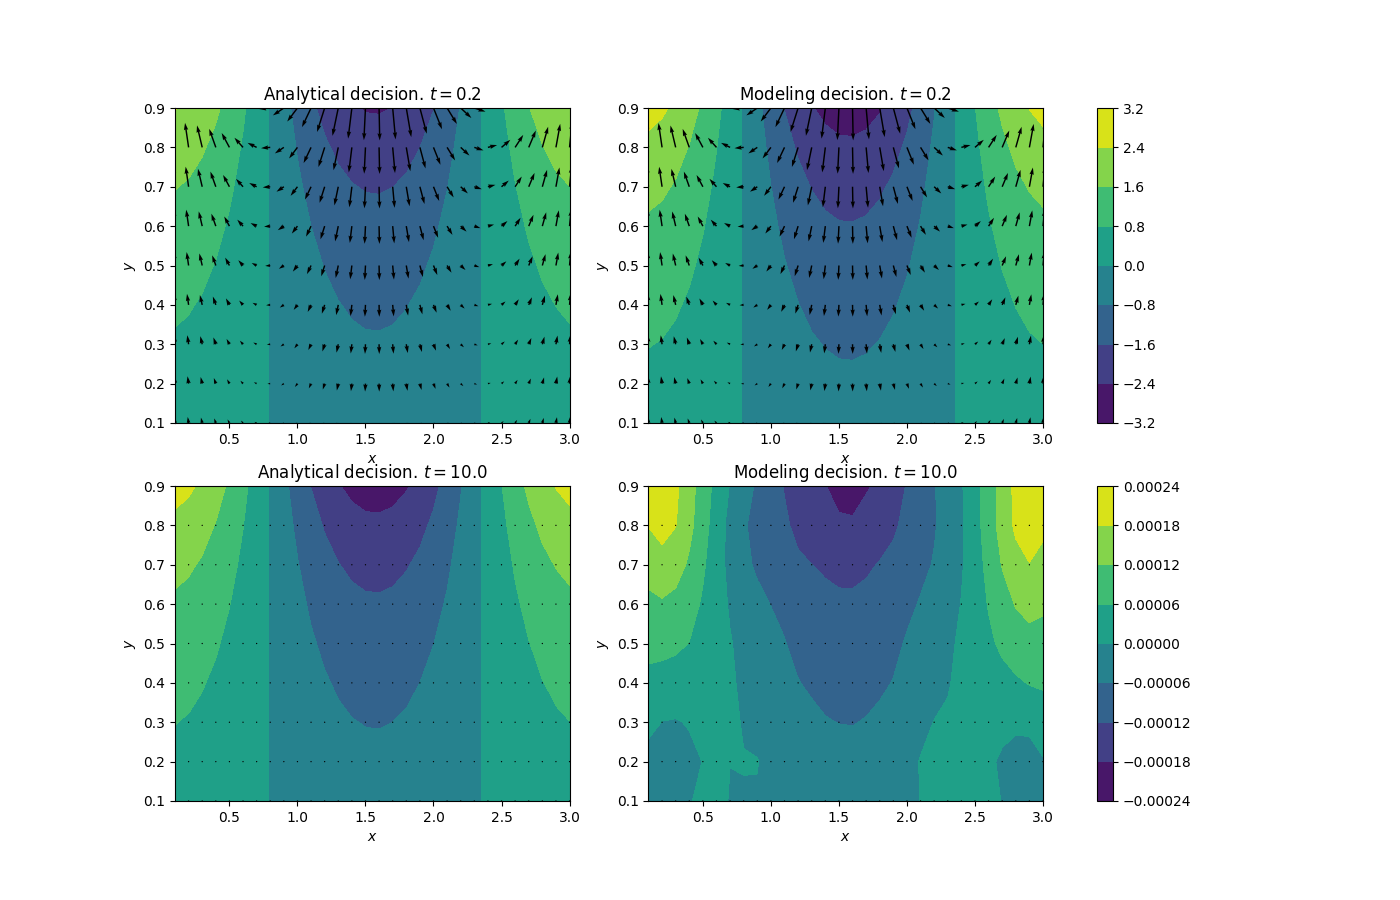
\includegraphics[scale=0.5]{Figure_1.png}
	\caption{Результати після $1$ та $100$ кроків.} \label{ris:1}
\end{figure}

Побудуємо графіки абсолютної похибки по крокам (рис. \ref{ris:2})

\begin{figure}[h]
	\center 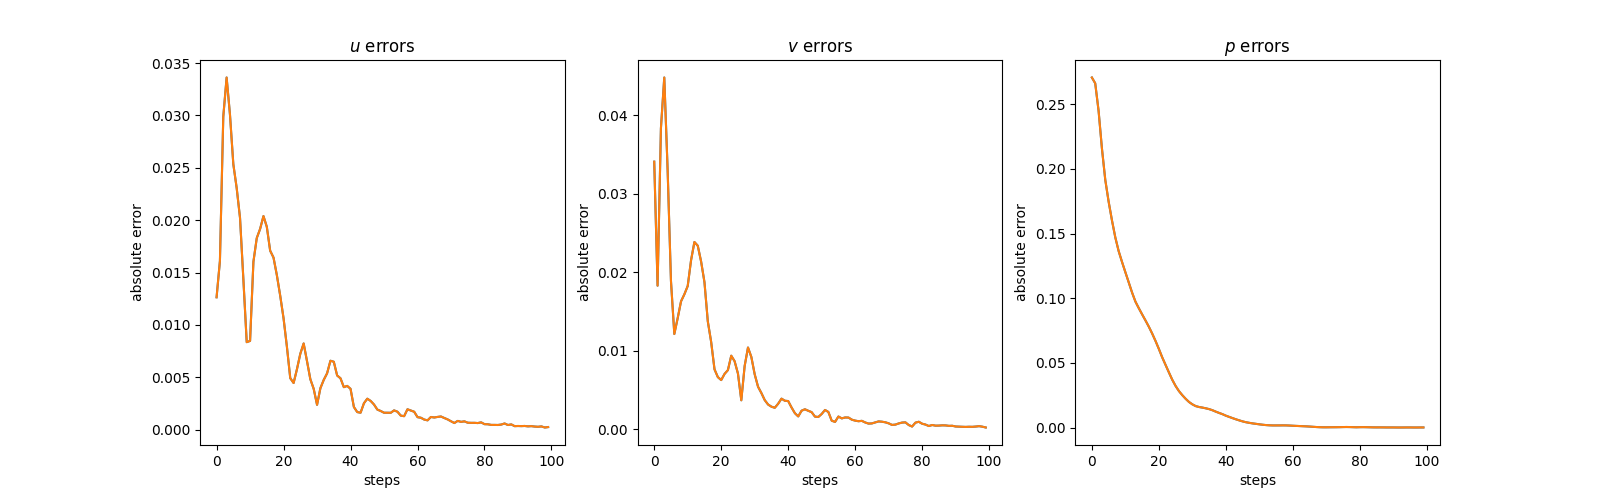
\includegraphics[scale=0.4]{Figure_2.png}
	\caption{Абсолютна похибка по крокам} \label{ris:2}
\end{figure}

Бачимо, що похибка для тиску $p$ доволі велика, вона зменшується з плином часу, оскільки зменшується саме значення тиску $p$. Також легко побачити, що і швидкість зменшується та прямує до нуля із збільшенням часу.

Анімацію можна знайти за посиланнями
\begin{itemize}
	\item Аналітичний розв'язок
	\item Чисельне моделювання
\end{itemize}

\subsection{Особливості моделювання}

Під час тестування програми я помітив цікаву поведінку програми при виборі дуже малого часового кроку $\tau = 0.0001$. При такому значенні кроку виникає помилка при обрахуванні значення тиску $p$. Це можна побачити на рисунку \ref{ris:3}.

\begin{figure}[h]
	\center 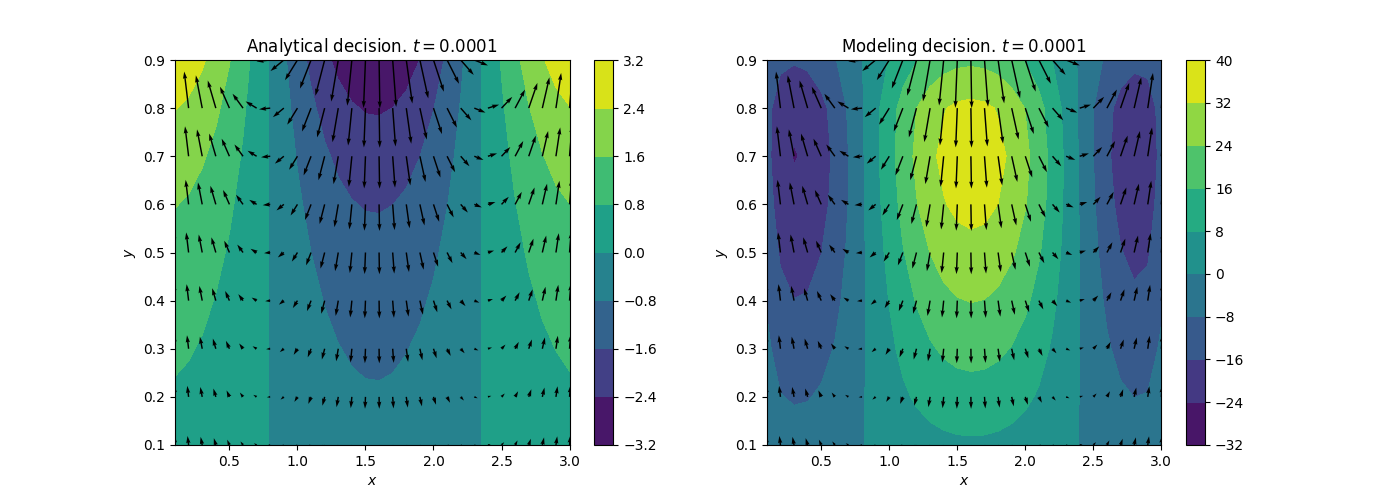
\includegraphics[scale=0.5]{Figure_3.png}
	\caption{Демонстрація помилки при обрахуванні $p$} \label{ris:3}
\end{figure}

Як видно з рисунка \ref{ris:3} виникає велика помилка при обрахуванні тиску. На мій погляд така помилка пов'язана із методом оновлення $p$ та малим значенням часового кроку $\tau$. 

Ми оновлюємо значення тиску за формулою (\ref{eq2.9}), де $S_i,j$ обраховується за формулою (\ref{eq2.5}). Легко побачити, що при дуже малих значеннях $\tau$ значення $S_{i,j}$ стає дуже великим, і навіть множник $h_x^2$ не може компенсувати цього.

Зрозуміло, що значення тиску при такій малій зміні часу не повинно сильно змінитися, але у формулу оновлення (\ref{eq2.9}) додається велике значення $S_{i,j}$, що спричиняє помилки.

Тому необхідно брати значення часового кроку $\tau$ приблизно рівне кроку по осі $x$ $h_x$.

\section{Висновок}

Було проведено чисельне моделювання в’язкої ньютонівської нестислої рідини. Знайшли деякі особливості методу моделювання.


\addcontentsline{toc}{section}{Література}
\begin{thebibliography}{}
	\bibitem{Rouch} Роуч П. Вычислительная гидродинамика. М. “Мир” 1980. с-616.
\end{thebibliography}

\end{document}
